%----------------------------------------------------------------------------------------
%	SLIDE 6.
%----------------------------------------------------------------------------------------
\begin{frame}
\frametitle{Linux használat}

\begin{columns}
	\column{0.45\linewidth}
	\begin{block}{Néhány fontosabb aspektus}
		\begin{itemize}
			\item POSIX standard
			\item Több, jobban karbantartott és sokoldalúbb szoftver
			\item Package manager szoftverek (apt, pacman, stb.)
		\end{itemize}
	\end{block}
	
	\uncover<2->{
	\begin{alertblock}{Zárógondolat}
		\begin{itemize}
			\item<3-> I use debian btw
			\item<4-> Köszönöm a figyelmet :)
		\end{itemize}
	\end{alertblock}
	}

	\column{0.5\linewidth}
	\begin{figure}
		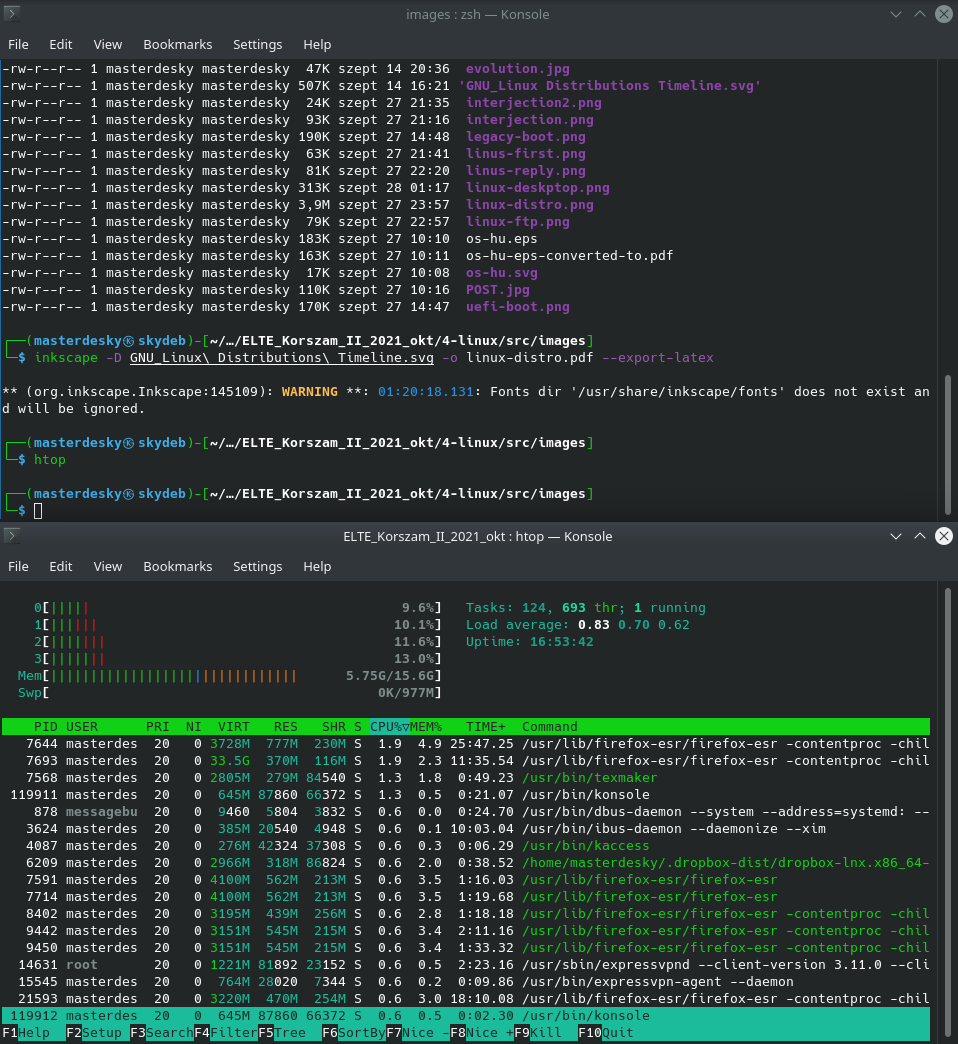
\includegraphics[width=1.0\textwidth]{images/linux-deskptop.png}
	\end{figure}

\end{columns}
\end{frame}

